\label{ch:collection}

% +===================+
% |      ROADMAP      |
% +===================+
%
% data Collection (falls performed and the hospital context)
% results
%

In order to further investigate the results obtained during the first experimentation session, a second testing trial was performed. This allowed the collection of additional data in order to draw conclusions in relation to the \textbf{feasibility} of the Electrodermal Activity analysis for classification purposes in the context of fall detection.

In this case, a commercial and publicly acknowledged device was employed in order to overcome the issues concerning the sensitivity to shocks and impacts of the BITalino device and, in addition, to acquire further bio-signals along with the Electrodermal Activity data.

\section{Selection of a High End Electrodermal Activity Sensor}\label{sec:movisens}

The device employed consists of the \textbf{EdaMove 4} sensor by \textbf{Movisens GmbH}, which is one of the most accurate and popular wearable devices aimed at the Electrodermal Activity measurement together with others such as the previously mentioned \textbf{Empatica E4}. In the following sections, a brief overview of the product and its features in proposed.

\subsection{Movisens GmbH}\label{subsec:movisens-company}

Movisens GmbH is a German company deemed as a global leader in ambulatory assessment solutions \cite{movisens}, which offers several services such as workshops, consults, customized products and software in order to support researchers and provide technologies for the healthcare sector.
The current catalog offers several instruments for data collection, integration, processing and analysis. More specifically, a list of the currently available products is reported in table \ref{toc:movisens-products}.

\begin{table}[H]
\centering
\begin{tabular}{ll}
    \hline
    Name                     &  Description \\
    \hline
    \textbf{Move 4}          & A 10-Axis IMU that integrates a temperature sensor \\
    \textbf{EcgMove 4}       & A Move 4 unit that integrates ECG data \\
    \textbf{EdaMove 4}       & A Move 4 unit that integrates EDA data \\
    \textbf{LightMove 4}     & A Move 4 unit that integrates the acquisition of ambient light measurement \\
    \textbf{SensorTrigger}   & A mobile solution for activity-triggered data logging \\
    \textbf{movisensXS}      & A mobile solution for Experience Sampling purposes \\
    \textbf{DataMerger}      & A desktop-based application for the integration of heterogeneous data \\
    \textbf{DataAnalyzer}    & A desktop-based application to analyze and report the acquired data \\
    \hline
\end{tabular}
\caption{List of the products implemented by Movisens GmbH}
\label{toc:movisens-products}
\end{table}

Additionally, the company provides several solutions that allow researchers and students to utilize the needed instrumentation by requiring a free, limited rent for a specific product. In this case, the company has consented a rental of the \textbf{EdaMove 4} sensor for the required period of time. 

\subsection{The EdaMove 4 Sensor}\label{subsec:edamove4}

Across all the products developed by Movisens, the EdaMove 4 is the one that implements measurement functionalities for the Electrodermal Activity. It consists of a 62,3 x 38,6 x 11,5 mm case with a 26 g weight \cite{edamove4} that provides a Micro-USB connection (in order to connect the unit to the \textit{Sensor Manager} software) and two snap-button connectors in order to attach the positive and negative electrodes. Moreover, a proper wrist band with pre-connected electrodes and specific mount points for the EdaMove 4 sensor allows the device to be worn seamlessly on the wrist or the ankle.


\begin{figure}[htp]
    \centering
    \subfloat[Electrodes Placement]{%
        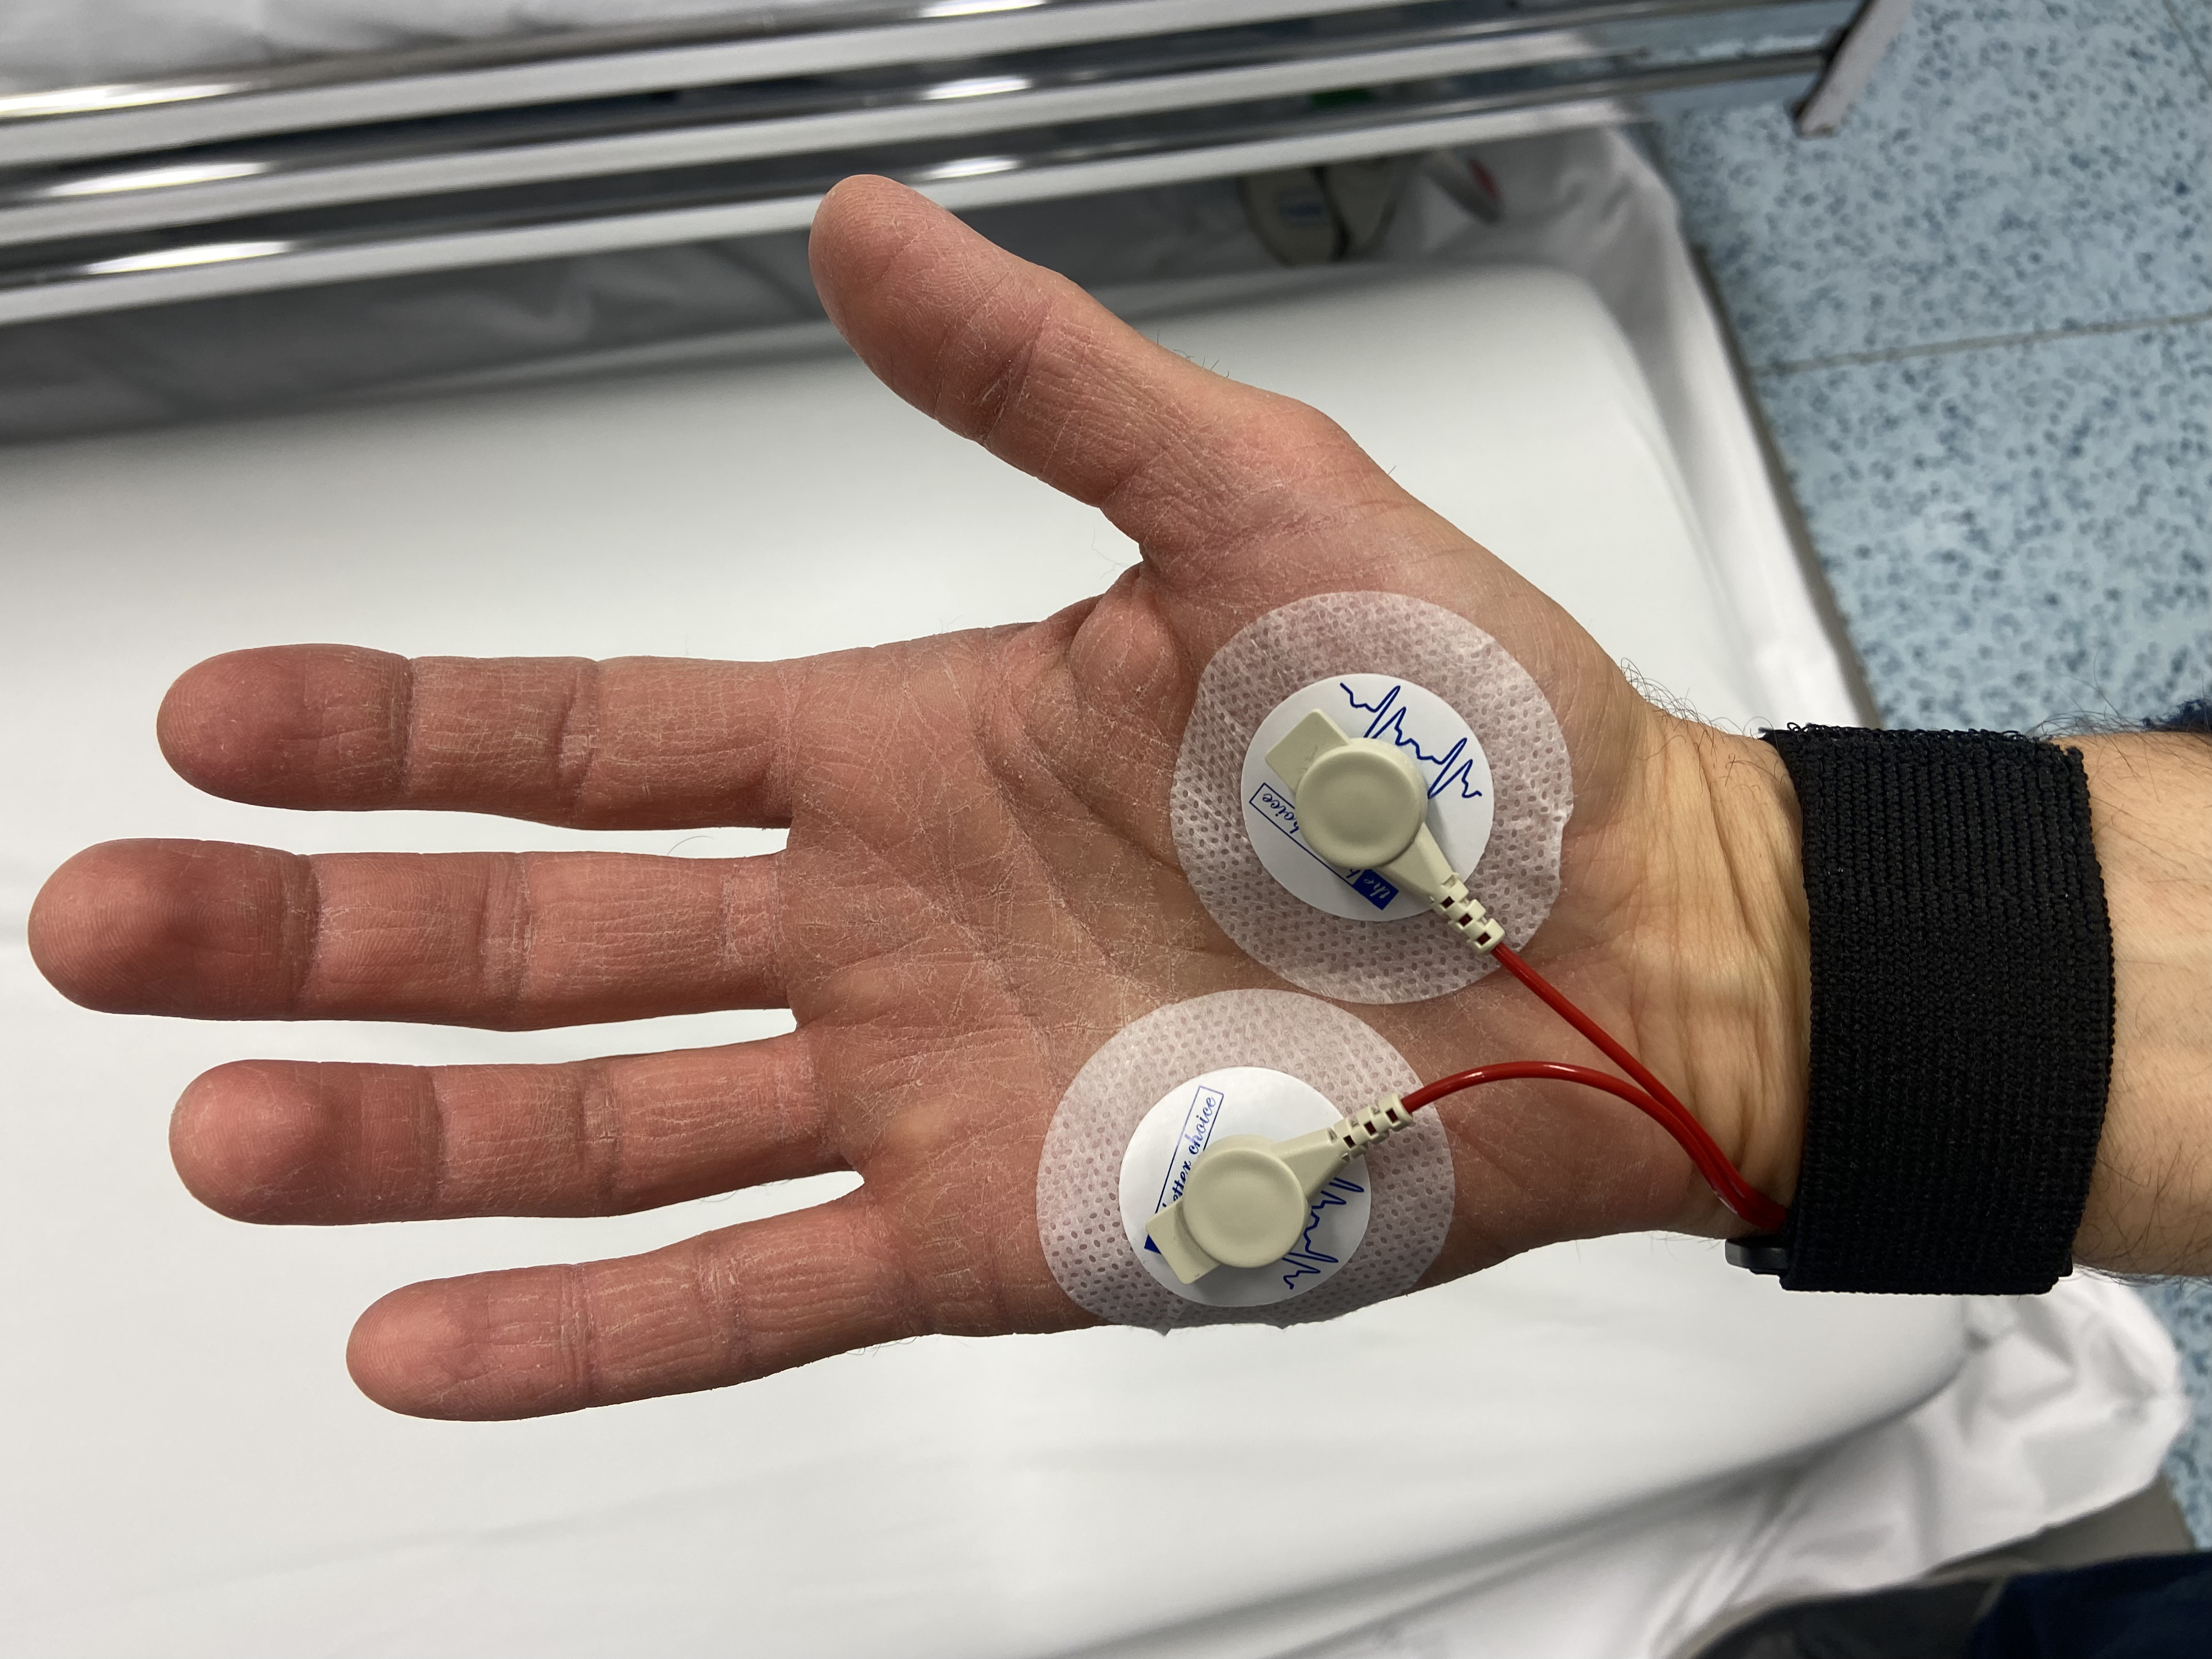
\includegraphics[width=0.4\textwidth]{./images/edamove1.jpeg}%
    }%
    \hfill%
    \subfloat[The Sensor Unit Employed]{%
        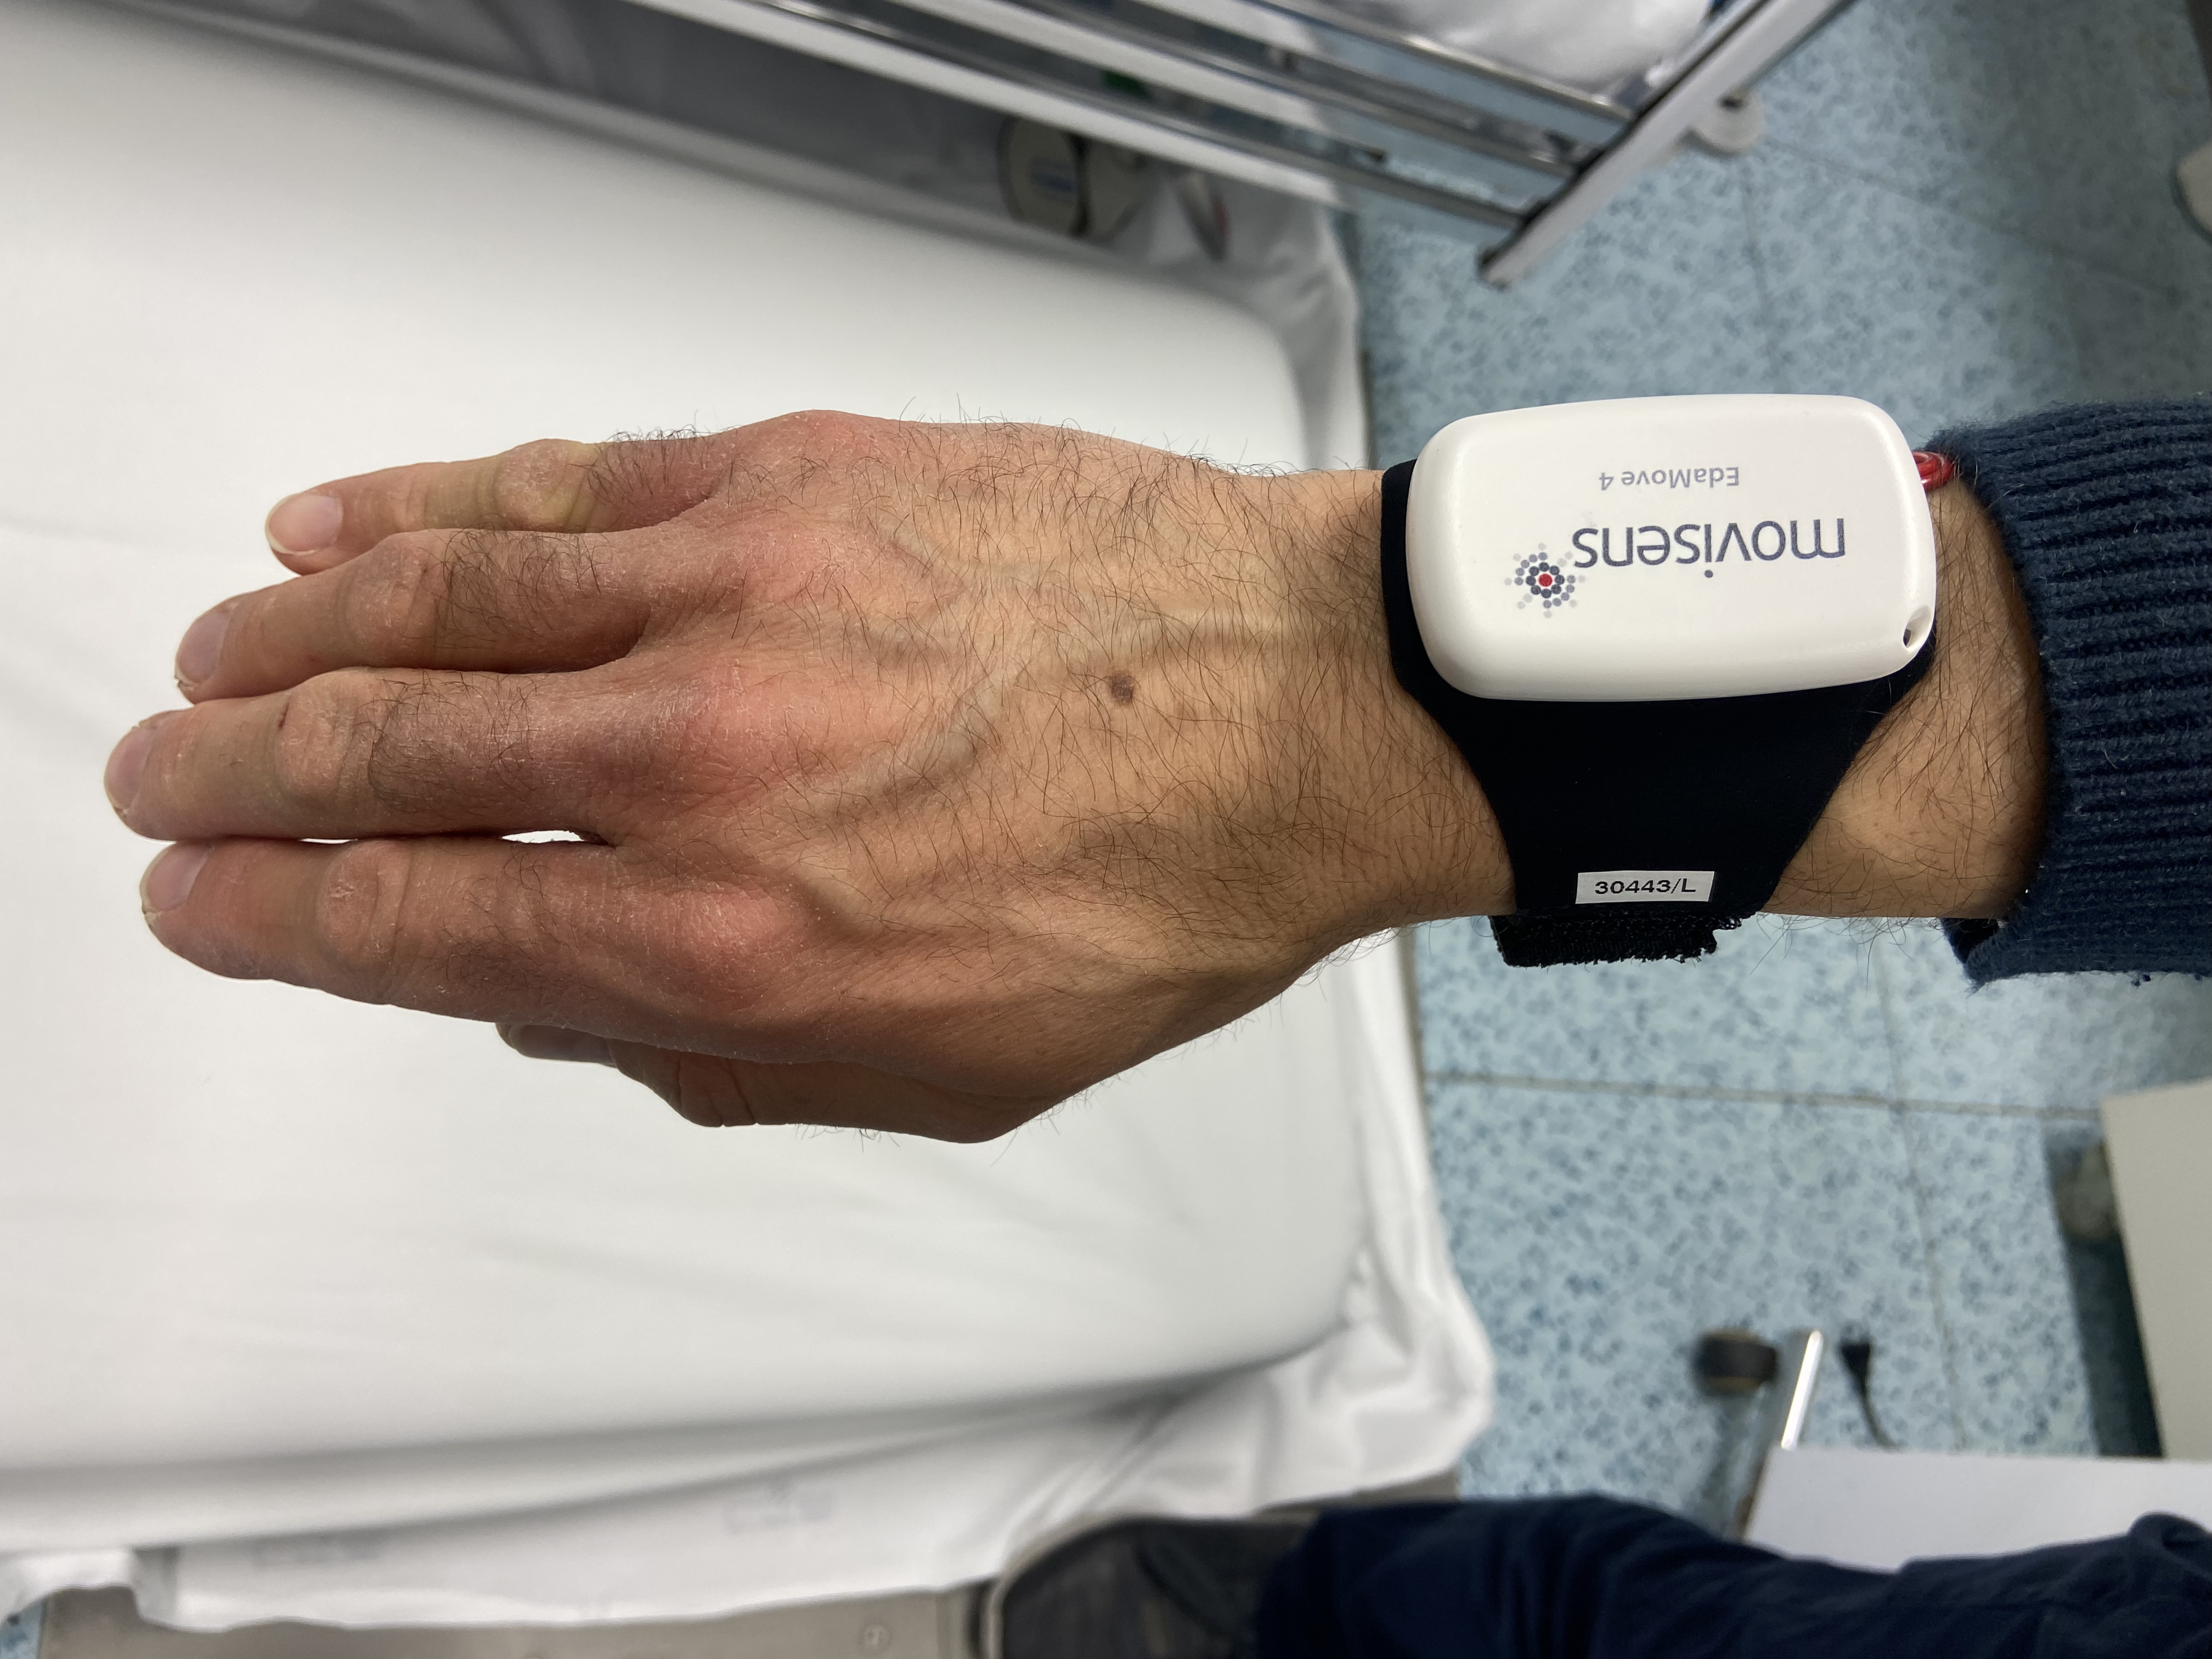
\includegraphics[width=0.4\textwidth]{./images/edamove2.jpeg}%
    }%
    \caption{The EdaMove 4 Sensor}
    \label{fig:edamovesensor}
\end{figure}

Other than acquiring EDA measurement, the unit also offers:

\begin{itemize}
    \item A \textbf{3D Accelerometer}
    \item A \textbf{Rotation Rate} sensor
    \item A \textbf{Pressure} sensor
    \item A \textbf{Temperature} sensor
\end{itemize}

More specifically, the unit implements an exosomatic acquisition technique by applying a standard voltage of 0.5 V DC. The internal Analog to Digital Converter provides a 14 bit resolution and the output rate corresponds to 32 Hz for a 8 Hz bandwidth.

Furthermore, the 3D accelerometer provides a $\pm$ 16 g range with an output rate of 64 Hz, while the rotation rate sensor offers a $\pm$ 2000 dps range, with a 64 Hz output rate and a 70 mdps resolution. The pressure sensor provides, instead, a measurement range between 300 and 1100 hPa, with a 8 Hz output rate and a 0.03 hPa resolution. Finally, the temperature sensor provides an output rate of 1 Hz.

The EdaMove 4 mounts a capacious Lithium battery which provides a constant 3.7 voltage and offers a continuous runtime of almost four days. An internal memory of 4 Gigabytes offers, instead, a maximum recording capacity of 4 weeks, allowing the usage of the sensor in varied contexts, from controlled experimentations to uncontrolled, domestic environments. 

Finally, the EdaMove 4 has been employed in several scientific publications that overall validated its functionalities and accuracy.

\subsection{Sensor Usage}\label{subsec:edamove4-usage}

In order to organise a measurement session and subsequently extract the obtained data, Movisens provides a specific software toolchain, which is cross-compatible between all the Move sensors. 

More specifically, the sensors can be configured through the \textbf{Sensor Manager} software, which allows the definition of personal data in relation to the individual and the specification of parameters such as the \textbf{duration} and the \textbf{start time} of the following measurement. Furthermore, the software detects whether the unit has non-retrieved measurements in its storage and provides functionalities to transfer the acquired dataset to the machine of the user. The data acquisition criteria can be configured in order to match one of the two modalities proposed: 

\begin{itemize}
    \item \textbf{Plain CSV} files
    \item \textbf{Unisens} File Format 
\end{itemize}

Besides Plain CSV is included as an option, the company highly suggests the usage of the Unisens format in order to exploit the functionalities that the standard implements. The latter is, in fact, compatible with both the \textbf{Unisens Viewer} and the \textbf{Data Analyzer} software. The first consists of a free and convenient tool that allows to plot and pre-process the raw data acquired (providing functionalities to remove unwanted sections and set specific markers in order to identify events of interest). The second one, instead, consists of a paid software that implements several algorithms and data processing techniques for the analysis of all the data acquired by Movisens products.

\subsection{The Unisens Data Format}\label{subsec:unisens}

One of the main difficulties that are required to be addressed when collecting data from multiple and heterogeneous sources is related to the storage and representation of the acquired information. More specifically, data can be retrieved at different sample rates or at specific time intervals and requires to be later synchronized e recomposed in order to be represented, analyzed and, eventually, classified. This problematic has been addressed in a multitude of different ways by researches. For example, as stated in \ref{subsubsec:upfall-technologies}, in the case of the UP-Fall dataset, a unique sample rate was defined in order to allow data synchronization from different sources. This strategy, however, required to lower the sample rate of certain devices which could have provided much more accuracy by configuring higher sample rates.

With these aims, the \textbf{FZI Research Center for Information Technology} and the \textbf{Institute for Information Processing Technology} at the University of Karlsruhe developed \textbf{Unisens}, a universal format standard that provides a shared criteria to collect multi sensor data \cite{unisens}. The latter is licensed under the LGPL license and provides the following abilities and features: 

\begin{itemize}
    \item Handling of continuous signals, as well as annotations and values
    \item Separate storage of multiple data channels
    \item Ability to synchronize data collected at various sample rates
    \item A layer of separation between raw data and meta information
    \item A flexible criteria to organise data in logical groups
    \item A human and machine readable meta information source file
    \item Ease of use, even in the case of embedded systems
\end{itemize}

The structure of a Unisens dataset involves the presence of several independent data sources stored as CSV or binary files which are, then, \textbf{aggregated} through a single XML file. The latter provides generic meta information in relation to additional sensor-related data, the initial time-stamp of the measurement, the source file of each data channel (with the required parameters in order to allow a correct parsing) and more. A brief example of the aforementioned file is reported below.

\begin{minted}{xml}

<?xml version="2.0" encoding="UTF-8" standalone="no"?>
<unisens comment="Description of the measurement" 
         duration="1186.0"
         timestampStart="2021-12-02T15:12:01.569"
         ...
         >
    <customAttributes>
        <customAttribute key="sensorLocation" value="right_wrist"/>
        ...
        <customAttribute key="sensorTimeDrift" value="-3.7783"/>
    </customAttributes>

    <signalEntry adcResolution="16"
                 comment="acc"
                 contentClass="acc"
                 dataType="int16"
                 id="acc.bin"
                 lsbValue="0.00048828125"
                 sampleRate="64"
                 unit="g">
        <binFileFormat endianess="LITTLE"/>
        <channel name="accX"/>
        <channel name="accY"/>
        <channel name="accZ"/>
    </signalEntry>
    ...
</unisens>
\end{minted}

As stated previously, the Movisens software toolchain provides a complete integration of the Unisens data format, which was therefore used in order to acquire and store fall detection related data. Additionally, Unisens provides support for common general-purpose programming languages such as \textbf{Python}, \textbf{Java}, \textbf{C\#} and \textbf{Matlab} other than offering the previously mentioned Unisens Viewer software, a desktop based application compatible with the Windows Operative System that allows users to interact with datasets through a graphical user interface. 

\section{Data Collection}\label{sec:edamove4-data-collection}

\subsection{Organisation of the Session}\label{subsec:session-org}

The data collection session was performed at the \textbf{Simulation Center} of the Santa Maria della Misericoria hospital in Udine and involved the participation of a single 49 years old male and healthy individual. A single EDA Move 4 sensor was employed and worn on the wrist of the dominant arm of the participant, as depicted in figure \ref{fig:edamovesensor}. All the activities performed have been reported in table \ref{toc:falls-performed-edamove}. Moreover, like for the previous session, it is important to note that all the falls were self-initiated and performed on purpose in a completely safe environment.

\begin{table}[H]
\centering
\begin{tabular}{ll}
    \hline
    Name         & Description \\
    \hline
    Bed          & Falling while getting up from a bed \\
    Sidewards    & Standing and subsequently falling on the side \\ 
    Bending      & Falling while picking up an object from the ground \\ 
    Standing     & Standing and subsequently falling slumping on the bed \\
    Front        & Standing and subsequently falling anteriorly  \\
    Backwards    & Standing and subsequenlty falling backwards \\
    \hline
\end{tabular}
\caption{List of the products implemented by Movisens GmbH}
\label{toc:falls-performed-edamove}
\end{table}

In this case, a \textbf{unique} and \textbf{continuous} measurement was acquired for the whole duration of the session. This strategy was adopted in order to provide the ability to analyze single event-related episodes as well as the whole evolution of the Electrodermal Activity throughout the entire duration of the experimentation. Moreover, timestamps were acquired in order to mark the beginning and the end of each fall in order to facilitate the subsequent process of separation of different events.

The acquired data (which also included information retrieved from the other sensors that compose the EdaMove 4) was, then, extracted and preprocessed in order to provide a single Unisens dataset for each one of the falls performed.





